\chapter{Objectifs de commande}
\minitoc
\label{chap:objectif}

\section{Contexte opérationnel}
Tout l'intérêt des drones est leurs capacités à se maintenir stabilisé sans intervention humaine. Ainsi, les opérateurs peuvent se concentrer sur la mission, sans devoir consacrer une grande attention au pilotage du drone. 

Les nombreux progrès dans les systèmes d'estimation état permettent de connaitre précisément l'orientation et la position des drones pour assurer la stabilisation, le guidage et la navigation. Les progrès sont lié à l'amélioration continue des capteurs, notamment des centrales inertielles (Inertial measurement Units, IMU), \nomenclature[]{\(IMU\)}{Centrales inertielles (\textit{Inertial measurement Units})} constitué d'un accéléromètre, d'un gyroscope et d'un magnétomètre. La Table \ref{tab:autopilote_ev} montre l'évolution des vitesses des microcontrôleurs (Microcontroller Unit, MCU) \nomenclature[]{\(MCU\)}{Microcontrôleurs (\textit{Inertial measurement Units})} embarqué sur les autopilotes et de la réduction du bruit des capteurs inertiel.
\begin{table}[ht]
    \centering
    \begin{tabular}{|c|c|c|c|c|c|}
        \hline
        Génération & Année & MCU & Vitesse & Capteur  & Bruit RMS \\
        \hline \hline
        \href{https://wiki.paparazziuav.org/wiki/Apogee/v1.00}{Apogee}  & 2013 & STM32F4 & 168 MHz & MPU-9150 & \begin{tabular}{ccc} Gyro : 0.06 dps \\
        Accel: 4 mg  \end{tabular}  \\
        \hline
        \href{https://wiki.paparazziuav.org/wiki/Chimera/v1.00}{Chimera} & 2016 & STM32F7 & 216 MHz &  MPU-9250 & \begin{tabular}{ccc} Gyro : 0.1  dps \\
        Accel: 8 mg  \end{tabular}\\
        \hline
        \href{https://wiki.paparazziuav.org/wiki/Tawaki/v1.10}{Tawaki 1} &2019 &  STM32F7 & 216 MHz  & ICM-20600 & \begin{tabular}{ccc} Gyro : 0.04 dps \\
        Accel: 1 mg  \end{tabular}\\
        \hline
        \href{https://wiki.paparazziuav.org/wiki/Tawaki/v2.01}{Tawaki 2} &2023 &  STM32H7 & 480 MHz & ICM-42688-P & \begin{tabular}{ccc} Gyro : 0.028 dps \\
        Accel: 0.70 mg  \end{tabular} \\
        \hline
    \end{tabular}
    \caption{Évolution des autopilotes paparazzi sur dix ans.}
    \label{tab:autopilote_ev}
\end{table}

Sur une période de dix ans, nous pouvons observer que les microcontrôleurs ont doublé leurs vitesses d'exécution, que les fabricants ont divisé par deux le bruit moyen sur les gyroscopes et par quatre le bruit moyen des accéléromètres.
Ces évolutions continues permettent une amélioration de l'estimation du drone utilisé pour la stabilisation. Il en résulte une stabilité accrue et de nouvelle possibilité pour la commande des drones.


\section{Contexte de la thèse}
De nombreux travaux ont été mener sur les \textit{tailsitters}, avec l'objectif de couvrir l'intégralité du domaine de vol. Ce dernier est constitué des phases de vol suivantes :
\begin{enumerate}
    \item Décollage vertical
    \item Transition entre le vol stationnaire et le vol d'avancement
    \item Vol d'avancement
    \item Transition entre le vol d'avancement et le vol stationnaire
    \item Atterrissage vertical
\end{enumerate}
Bien que l'on puisse observer une symétrie dans la phase \raisebox{.5pt}{\textcircled{\raisebox{-.9pt} {1}}} et \raisebox{.5pt}{\textcircled{\raisebox{-.9pt} {5}}}, qui correspondent au décollage et à l'atterrissage vertical, une différence fondamentale est observé. Lors du décollage, la vitesse du drone engendrera un flux d'aire sur l'aile orienté dans le même sens que le flux d'aire généré par les hélices. Cependant, lors de l'atterrissage, le flux d'air va se trouver inversé, le drone doit descendre, ce qui engendre une vitesse opposée à la direction du flux d'air des hélices. Cette inversion génère une instabilité qui doit être compensé par le contrôleur.

\begin{figure}[ht]
    \centering
        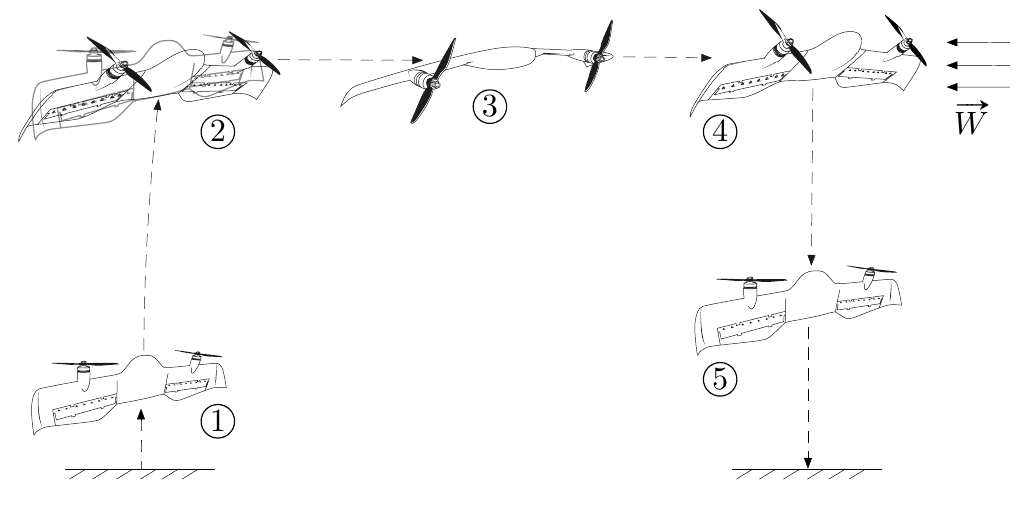
\includegraphics[width=0.8\columnwidth]{figures/darko_transition.png}
        \caption{Phase de vol d'un drone \textit{tailsitters}, DarkO.}
        \label{fig:darko_flight}
\end{figure}
Le vecteur $\overrightarrow{W}$ représente la perturbation de vent qui peut affecter le vol sur l'intégralité des cinq phases de vol.

methode sans modèles 




\todo{rejet de perturbation, model based control}


\section{Résumée}